% \subsection{Research Thrust 1: Execution Reconstruction}
% \label{sec:thrust1}

% \begin{wrapfigure}{R}{0.42\textwidth}
% \centering
% 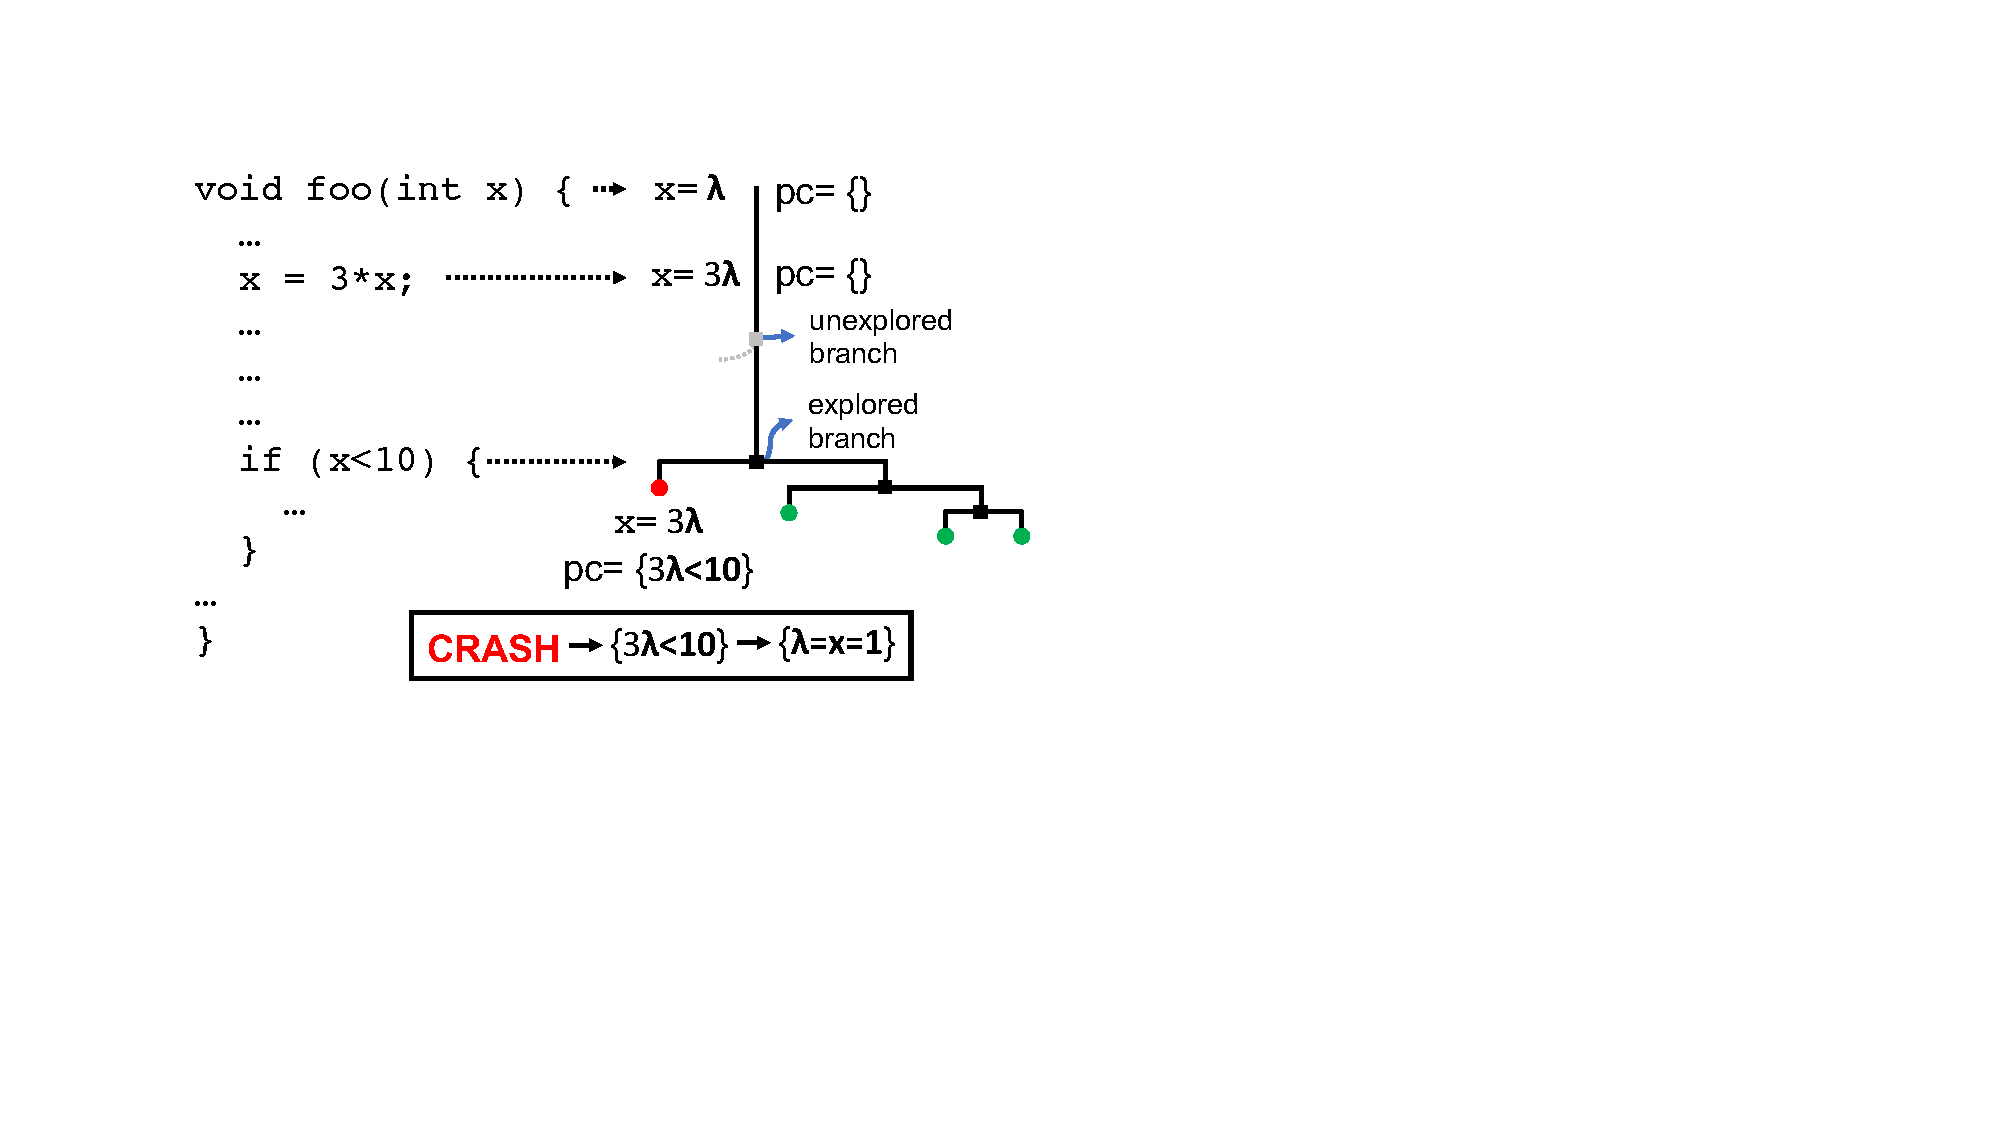
\includegraphics[width=\linewidth]{Figures/symbex.pdf}
% \caption{Symbolic execution}
% \label{fig:symbolic}
% \end{wrapfigure}

% In \S\ref{sec:preliminary}, we showed that \textit{\textbf{existing bug reproduction techniques are not simultaneously} \textbf{effective, accurate, efficient and non-invasive}}, and that \textit{\textbf{latent bugs}} \textit{\textbf{pose great difficulty for bug reproduction}}. This thrust will develop techniques that address these challenges for \textit{sequential} programs. 

% \subsubsection{Background: Symbolic Execution}
% \label{sec:background}
% Symbolic execution~\cite{king:symbolic,klee,Chipounov11,godefroid:sage,boyer:symbolic} executes a program with \textit{symbolic} inputs (as opposed to concrete)  to explore the input space. In Fig.~\ref{fig:symbolic}, {\tt foo} is executed with the symbolic value $\lambda$. During execution, values are updated (e.g., $x = \lambda$). When a branch condition with a symbolic value is encountered, the execution \textit{forks} into two independent states. Each state tracks the \textit{path condition} (pc), which led to previous forks. The solution to a path condition is a concrete assignment to symbolic variables by a constraint solver~\cite{stp, z3}. The solver is invoked when an event of interest (e.g., a crash) occurs and tries to find a satisfying variable assignment that makes the path constraint hold true (e.g., $x=\lambda=1$).

% \textit{Symbolic execution has two key limitations}. First is \textit{path explosion}, which arises because the number of states that needs to be symbolically executed is exponential in the number of branches that depend on symbolic inputs. The second challenge is \textit{constraint solving complexity}, which increases as the explored path deepens and the path constraints become increasingly more complex.

% \subsubsection{Task 1.1: Trace-Driven Symbolic Execution} 
% \label{sec:task11}
% In this task, we will develop \textit{trace-driven symbolic execution} as the key novel technique to reproduce failing executions. \textbf{\textit{We will address the path explosion challenge using control flow traces gathered from production executions}} using \textit{efficient} and \textit{non-invasive} hardware support (i.e., 1\%-3\% overhead~\cite{ninjaetm,snorlax}) such as ARM ETM~\cite{armetm} or Intel PT~\cite{intelpt}, which are present in most modern systems. When a program crashes, hangs, or triggers an assertion, the trace will be shipped back to the server (via the coredump) and used to drive symbolic execution down a \textit{single} path to reproduce the bug. In this task, we will continuously monitor the control flow of programs similar to prior work~\cite{h3,retracer,racemob,gist,snorlax}. We will keep a compact trace in a ring buffer for \textit{efficiency} (rather than flushing the buffer to persistent store when full~\cite{h3}), so the reproduced execution may be a part of the entire execution (akin to MicroX~\cite{microx} and UC-KLEE~\cite{ucklee}), a limitation we will overcome in the next two tasks. 

% Constraint solving, which is an NP-complete problem~\cite{npcomplete1,npcomplete2}, is still a challenge. We will address this using two new approaches: (1) First, we will use concrete data recovered from the core dump to simplify constraints, (2) Second, if the solver cannot solve the path constraint (e.g., in 1-2 minutes as in prior work~\cite{rept}), we will incrementally remove clauses from the path constraint (by assuming they are True) to simplify it. Our insight is that since the control flow trace is from a real execution, the path constraint, which is in conjunctive normal form ($clause_1 \wedge .... \wedge clause_n$) should be satisfiable, but the solver falls short. Removing a clause would mean that we will not be able to determine the values of certain data values computed during the failing execution. This approach is \textit{effective}, but may slightly lower \textit{accuracy}. To minimize this adverse effect, we will remove clauses with the least number of variables until the remaining path constraint is satisfied. We will also apply this removal heuristic judiciously to ensure we can recover above 90\% of data values used by the program along the trace to match the accuracy of REPT~\cite{rept}, but \textit{greatly exceed its effectiveness due to reconstructing a much longer-running execution}.

% \noindent \textit{\noindent \textbf{Prior and Preliminary Work.}} In a prior presentation~\cite{hase}, we discussed the possibility of using hardware support to guide symbolic execution. As preliminary work, we modified Klee~\cite{klee} to record the control flow (simulating real hardware) of a failing execution in SQLite~\cite{sqlite}, a popular database. We replayed this trace of more than \textit{a million} instructions and generated an input that reproduces the crash with 100\% accuracy in under a minute. In contrast, we used execution synthesis~\cite{esd} (i.e., static analysis + Klee) for 24 hours, and could not reproduce this bug. These results are \textit{very encouraging} when compared with the state-of-the-art REPT~\cite{rept}, which can reconstruct executions within a 100,000 instruction window with 90\% accuracy.

% \noindent \textit{\noindent \textbf{Related Work.}} Concolic (hybrid concrete-symbolic) execution~\cite{cute,dart} collects constraints along a path when a program is run with a \textit{known} input. These constraints are then modified to generate further test inputs that explore alternate program paths. The main difference to our approach is that we do not assume knowledge of program inputs, but rather try to infer them using the control flow trace. S2E~\cite{Chipounov11} symbolically executes select program components, but may be unable to progress if it cannot solve path constraints, whereas we propose a way to progressively simplify constraints to achieve forward progress. 

% \subsubsection{Task 1.2: Hybrid Slice Computation via Program-Specific Monitoring}
% \label{sec:task12}

% In this task, we will introduce a new construct called the \textit{hybrid static/dynamic program slice}. A hybrid slice is an approximation of the instructions leading to a bug that gets incrementally more \textit{accurate} as users run programs. In the next task, we will use symbolic execution along the hybrid slice to reproduce bugs in long-running executions and improve \textit{effectiveness}. We will build the hybrid slice using the failure report and by monitoring program-specific information from \textit{successful executions}. Crucially, although we can leverage bug recurrences, we do not rely on this. \textbf{\textit{The key insight is that reconstructing a buggy execution along the hybrid slice should be sufficient for debugging, and there is no need to recreate the exact bug that occurred in production}}.

% %Selective execution monitoring will quickly gather information pertinent to the bug. We will reconstruct a more accurate failing execution along the hybrid slice.


% We will start by computing a static interprocedural backward slice~\cite{slicing} from the failure point (e.g., segmentation
% fault, failed assertion, etc.). This slice will contain all the instructions that \textit{may} affect the operands of the failing instruction. To compute the static slice, we will use an inclusion-based alias analysis~\cite{andersens} built atop LLVM~\cite{lattner2004llvm,lattner2008llvm}. For C/C++ programs we will generate LLVM bitcodes using clang~\cite{clang}; for other languages or when the source code is not available, we will explore using binary to LLVM translation~\cite{mctoll,revnic} or relying on specialized static analysis frameworks (e.g., Chord~\cite{chord} for Java).

% \begin{wrapfigure}{R}{0.14\textwidth}
% \centering
% 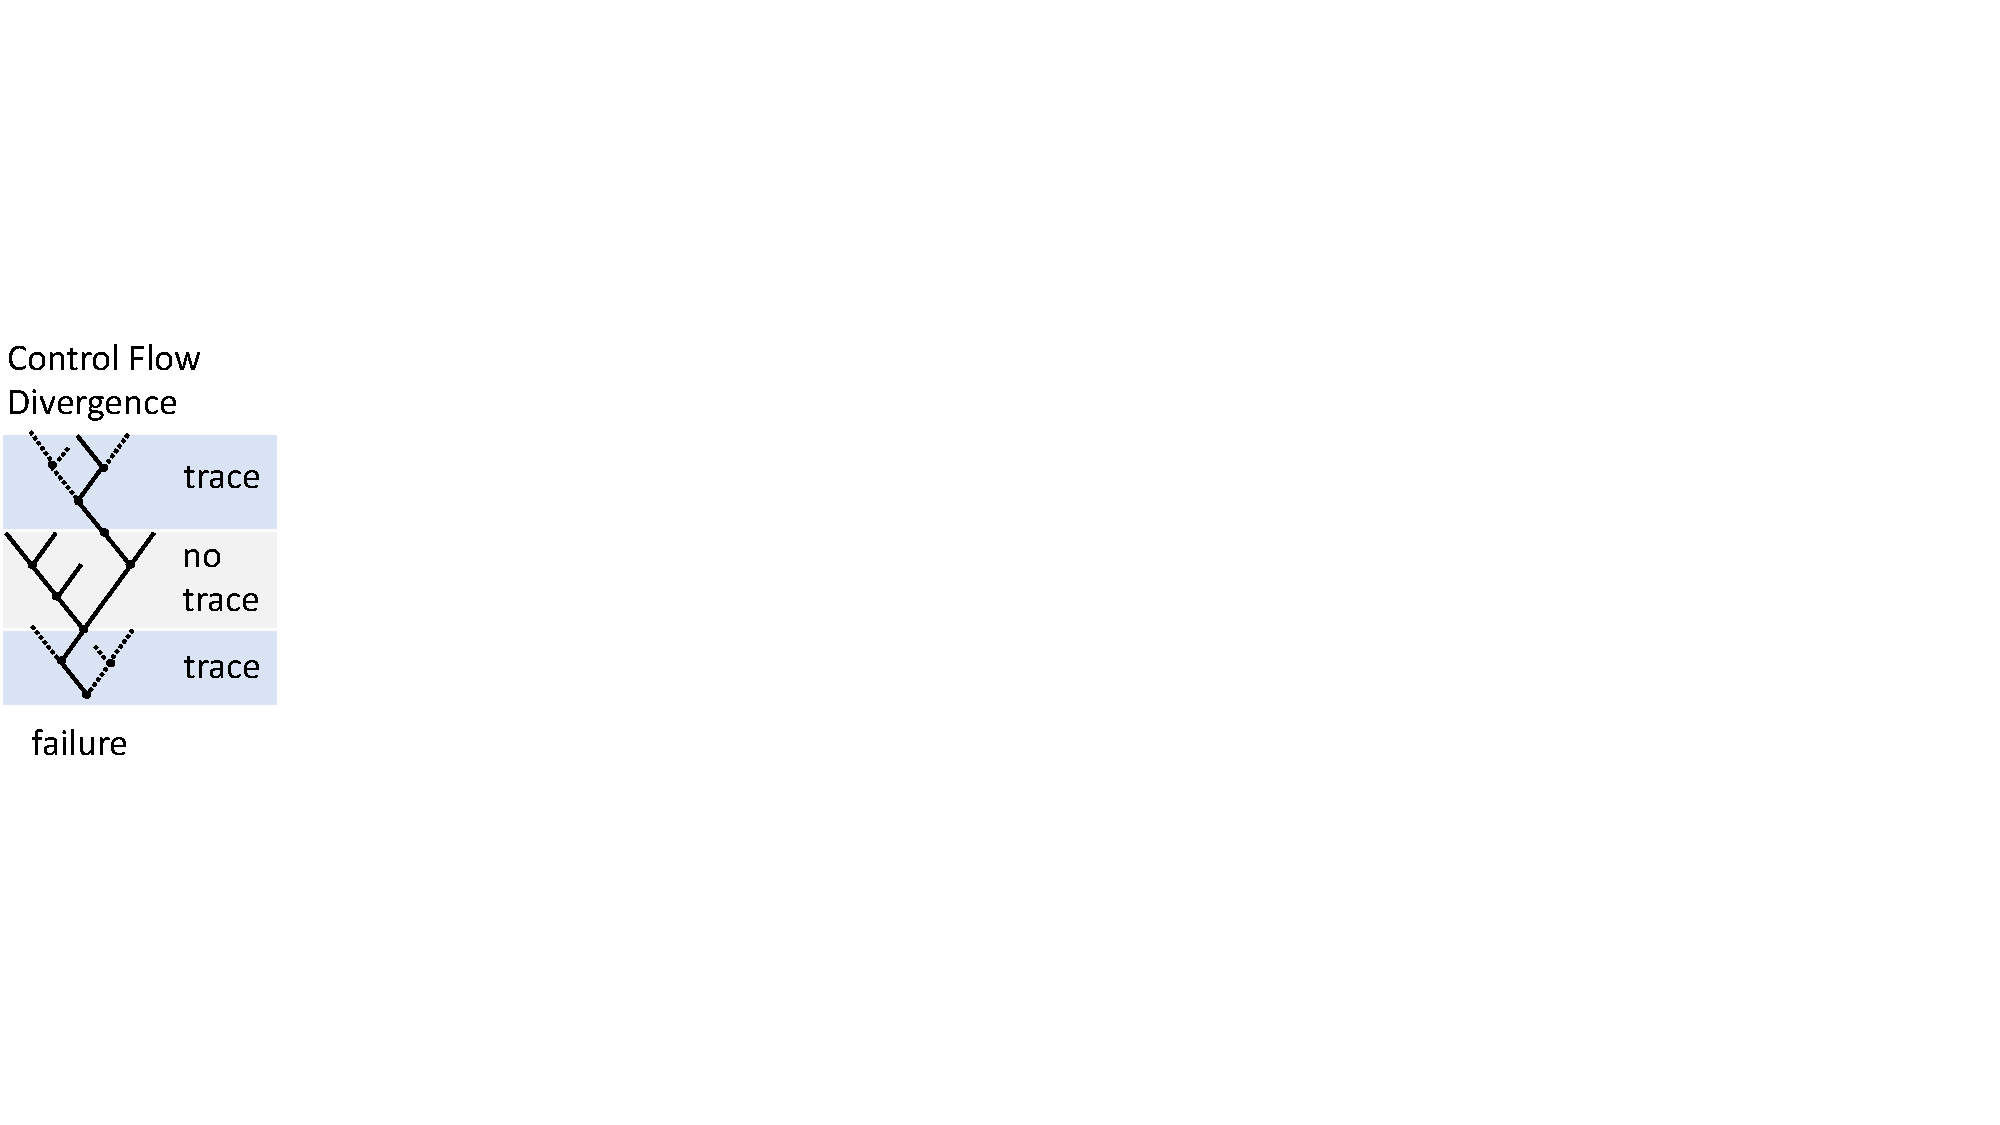
\includegraphics[width=\linewidth]{Figures/slicing-challenges-1.pdf}
% \caption{Fixing control flow divergence}
% \label{fig:slicing-challenges-1}
% \end{wrapfigure}

% Theoretically, it is possible to reconstruct an execution along the static slice as prior work has done for individual functions~\cite{choppedsymbex} (i.e., \textit{intraprocedurally}). This is harder when the static slice spans the entire program (i.e., \textit{interprocedurally}) and contains many inaccuracies due to the instructions that do not pertain to the bug, making symbolic execution ineffective. We will address key challenges that cause inaccurate static slices:

% First challenge is the large number of potential control flow paths that diverge backward from the failure, which we will address by using the control flow trace from the \textit{failing execution}. As opposed to T1.1 that continuously monitors the control flow in a ring buffer, in this task, we will switch to a bursty tracing policy~\cite{burstysampling} that periodically turns control flow tracing on and off to record subsequences of branches. For each subsequence, we will remove from the static slice, instructions that are not in the subsequence (i.e., dashed lines in Fig.~\ref{fig:slicing-challenges-1}). The key idea behind bursty tracing is to better tame the backward control flow divergence problem than a policy that continuously monitors branches. Since the trace is collected during the actual buggy execution, this removal will not impact soundness. 

% \begin{wrapfigure}{L}{0.39\textwidth}
% \centering
% 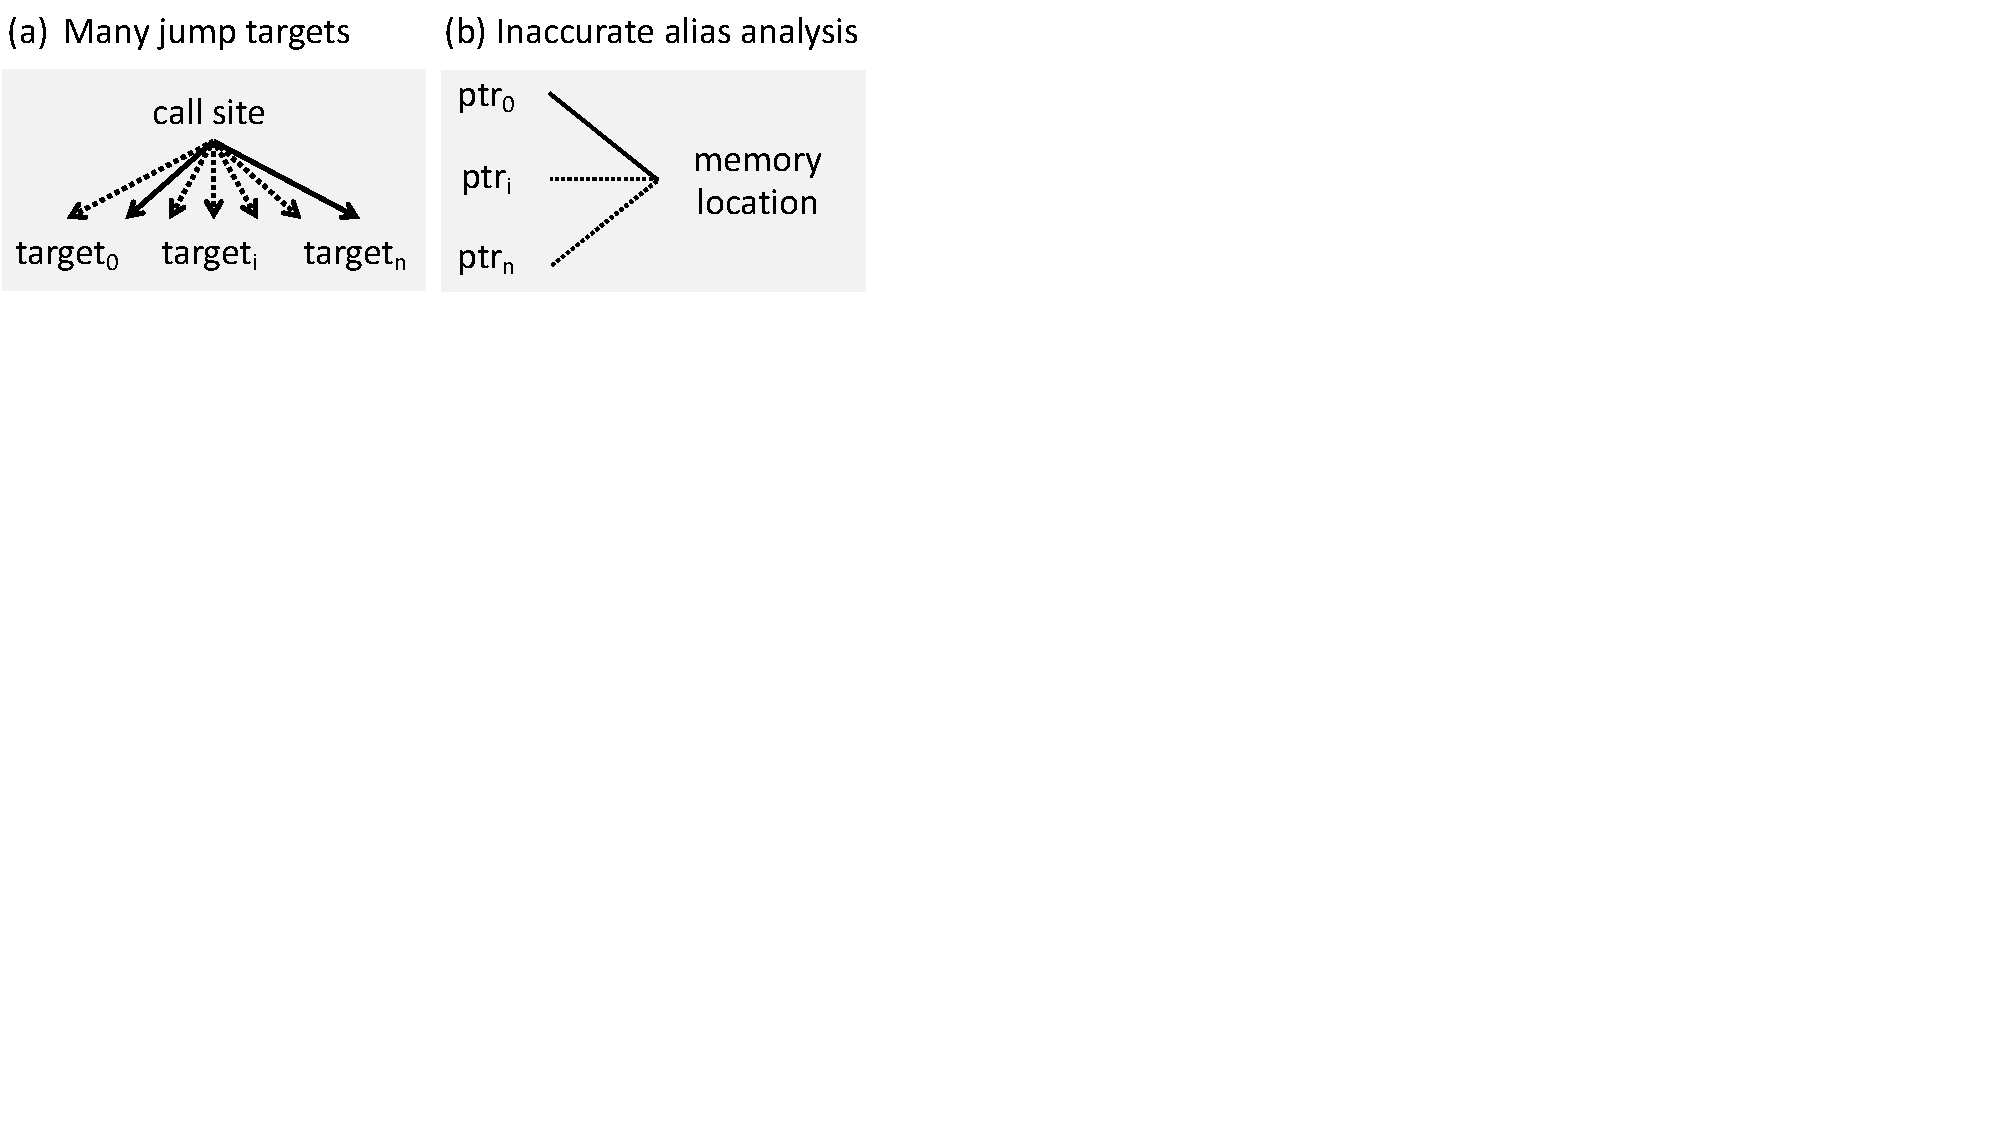
\includegraphics[width=\linewidth]{Figures/slicing-challenges-2.pdf}
% \caption{Call site and aliasing inaccuracies}
% \label{fig:slicing-challenges-2}
% \end{wrapfigure}

% The second challenge is the large number jump targets at indirect function call sites, which we will address by monitoring actual jump targets during subsequent successful (and potentially failing) executions (solid arrows in Fig.~\ref{fig:slicing-challenges-2}.a). For this, we will use targeted control flow monitoring (in a range of program counters) supported by Intel~\cite{intelpt} and ARM~\cite{armetm}. This information will be kept in a dedicated memory region separate from the region used for bursty tracing explained above.

% The third challenge is that interprocedural alias analysis causes many pointers to inaccurately point to the same memory location. We will address this issue by tracking the addresses accessed by pointers (e.g., $ptr_0...ptr_n$) in successful (and potentially failing) executions. We will use data tracing features of modern hardware (PT\_WRITE~\cite{intelptwrite} on Intel processors since Kaby Lake~\cite{kabylake} and ARM ETM~\cite{armetm}). We will use binary instrumentation~\cite{dynamorio,dynamoriosite} to non-invasively instrument programs with data tracing instructions. As users execute programs, we will learn which pointers actually alias (solid arrows in Fig.~\ref{fig:slicing-challenges-2}.b). We will then remove from the static slice instructions that were included in the slice due to inaccurate alias analysis.

% Removing jump targets and unobserved aliases from the static slice can theoretically lead to unsoundness. We used a similar technique in the past~\cite{racemob,gist} with no effect on soundness in practice. Regardless, we will continue monitoring programs as they execute to improve soundness as much as possible. 

% The hybrid slice can contain multiple paths and represent an over-approximation of the original buggy execution. Symbolic execution will have to explore multiple program paths to synthesize a failing execution, but the number of paths will be much fewer than during regular symbolic execution.

% \noindent \textit{\textbf{Latent Bug Hypothesis.}} Intuitively, even if the failure and its root cause are far apart in time and/or space, the state that causes the failure will be identical at the failure site and the root cause site. This simple hypothesis presents an opportunity for tackling latent bugs. When this hypothesis holds and if we can recover data and control flow along the hybrid slice---whose scope is the \textit{\textbf{entire program}}---, we will be able to reproduce the underlying data and control flow dependencies that result in a latent bug.

% \noindent \textit{\textbf{Prior and Preliminary Work.}} In prior work~\cite{gist}, we used hybrid static/dynamic analysis for failure diagnosis~\cite{snorlax,gist} and data race detection~\cite{racemob}. We relied on software instrumentation or a limited number of hardware breakpoints, which was invasive and ineffective. As preliminary work, we implemented a tool to determine the extent to which recording branch targets can impact static slices. We randomly selected 10 bugs in Apache httpd~\cite{apache-httpd} and computed a static slice from the failure point (using a static slicer~\cite{giri} we built in prior work~\cite{gist}). This resulted on average 270.7 potential call targets per each indirect call site in the slice. After running httpd tests~\cite{apache-bench}, the average number of targets per indirect call site was reduced to 2.1, an encouraging 100$\times$ reduction. We also verified that this reduction did not come at the expense of ineffectiveness (i.e., unsoundness): the buggy code was still present in the hybrid slice for all the 10 bugs.

% \noindent \textit{\textbf{Related Work.}} Our notion of a hybrid slice is different than prior work~\cite{hybridslicing} that uses the dynamic information in a debugging session to improve the accuracy of static slices. In contrast, we aggregate dynamic execution information from multiple successful executions to reason about a failing execution.

% \subsubsection{Task 1.3. Adaptive Symbolic Execution} 
% \label{sec:task13}
% In this task, we will adaptively monitor data values in failing and successful (primarily) executions to help symbolic execution synthesize more complex and longer-running executions (e.g., for latent bugs) along a hybrid slice. As mentioned in T1.2~(\S\ref{sec:task11}), a hybrid slice contains multiple paths, which can be challenging for symbolic execution. Moreover, constraint simplification from Task 1.1~(\S\ref{sec:task11}) may not be acceptable due to accuracy requirements, or, it may not help the solver. We address these challenges via \textit{adaptive symbolic execution}, a new technique to adaptively monitor data values a program uses to guide constraint solving heuristics. The key idea is to \textbf{\textit{record data values that will help constraint solving}} in symbolic execution. This technique \textbf{\textit{adaptively modifies the values monitored in production to satisfy the path constraint}}.

% Our first approach targets bugs that recur in production. We will leverage a heuristic called dynamic largest individual sum~\cite{satheuristic} (DLIS), to help us identify which data values used by the program should be recorded along the hybrid slice (which will be already computed after the initial failure) to help with constraint solving. DLIS allows ranking the variables in the path constraint in terms of the number of unsatisfied clauses that the variable would satisfy. Intuitively, prioritizing the recording of data values that help satisfy more clauses in the path constraint should allow quickly finding a satisfying assignment to the path constraint. In a long-running execution of a real program, we expect that we will not be able to record all the variables, therefore we need a practical limit as to how many variable values we can record. We will start by reserving a dedicated space to record this information in addition to the buffers that will be used in T1.1 and T1.2. By default, these buffers will each be less than a megabyte, but we will explore different buffers sizes and their impact on effectiveness, accuracy and efficiency (\S\ref{sec:evaluation}).

% Alas, the bug may not recur in production, in which case we will gather data values from successful executions. We will use these data values to reproduce failing executions by developing new constraint solving heuristics. A data value recorded from a successful execution can be used in two ways: (1) First, the value can help solve a path constraint in a failing execution. After all, failing and successful executions share many attributes and certain data values may be common in both, (2) Second, the value is only feasible for a successful execution and does not help reproduce the failure. We will determine the second case when the recorded value does not satisfy the path constraint. We will use such values to form a \textit{global counterexample cache}. Symbolic execution engines like Klee~\cite{klee} use a counterexample cache for a given symbolic execution run, where they incrementally cache values that are known to not satisfy the path constraint (Klee reports $40\%$ speedup thanks to its counterexample cache~\cite{klee}). \textit{Our key novelty is extending this notion to multiple program executions where we cache values that we know do not satisfy the path constraint.}

% We will also use the global counterexample cache to develop different constraint solving heuristics. In particular, we will use the values in the counterexample cache to generate dynamic invariants~\cite{daikon}, which we will use to inform constraint solving heuristics. For numerals (e.g., integers, floats etc.), we will use interval-based heuristics. For example, if the counterexample cache from successful executions contains values 10 and 1000 for a variable $x$, we will inform the solver to first attempt values that are outside the range $10 < x < 1000$, i.e, $x \leq 10$ or $x \geq 1000$. For strings, we will use a specialized solver~\cite{hampi} that is capable of efficiently maintaining constraints and counterexamples over string variables.

% %Finally, we will also target recording generic information that is known to cause path explosion such as loop upper bounds that depend on program inputs, as well as certain symbolic pointers that can not be dereferenced without causing path explosion. We will identify these sources of path explosion during trace-driven symbolic execution (Task 1.1.).

% \noindent \textit{\textbf{Preliminary Work.}} To determine whether the global counterexample cache can help speed up symbolic execution, we modified the counterexample cache in Klee to persist counterexamples across executions. We then used coreutils' test harness~\cite{coreutils-test} to populate the counter-example cache. With the global counterexample cache, Klee was able to discover the same bugs as baseline Klee 2.5$\times$ faster.

% \subsubsection{Potential Challenges and Mitigation Strategies} We envision the following challenges may arise: \textit{\textbf{Multiple Bugs.}} If we try to reproduce multiple bugs in a given system simultaneously, we will rely on the large number of users to form clusters, where each cluster is responsible for reproducing a given bug. We used a similar technique in prior work with great effectiveness~\cite{gist,racemob}.

% \noindent \textit{\textbf{Privacy.}} Reconstructing user executions and data has privacy implications. We rely on symbolic execution to reconstruct \textbf{an} execution that manifests a given failure (and not \textbf{the} execution), which mitigates some of the privacy concern as observed by prior work~\cite{betterbug}. However, we will rely on some data values from real executions (e.g., the core dump). Existing error reporting systems~\cite{ubuntuApport,wer} address similar issues by asking users to opt-in. In addition to adopting an opt-in policy, we can rely on trusted execution environments (e.g., Intel SGX~\cite{anati2013innovative,mckeen2013innovative} or ARM TrustZone~\cite{alvestrustzone}) to reproduce bugs while preserving user privacy.

% \noindent \textit{\textbf{Constraint Simplification.}} As we mentioned, removing clauses from the path constraint will result in executions that are partially reconstructed. The memory state that is unknown may make it hard for a developer to debug the program. In that case, we can rely on the developer to request a new simplification strategy that will reconstruct the desired memory state and leave some other state unknown.
